\subsection{Secciones de la página web}

    En esta subsección se dará una breve explicación de cada sección de la plataforma web y se acompañará de una imagen.

    \begin{itemize}
        \item Home

        Es la página web que visualiza un usuario no logueado en el sistema donde puede registrarse en ella, recordar la contraseña en caso de que la haya olvidado o registrarse.

        Además, también se muestra información pública sobre los objetivos, la misión y la visión del proyecto.

            \begin{figure}[H]
                \centering
                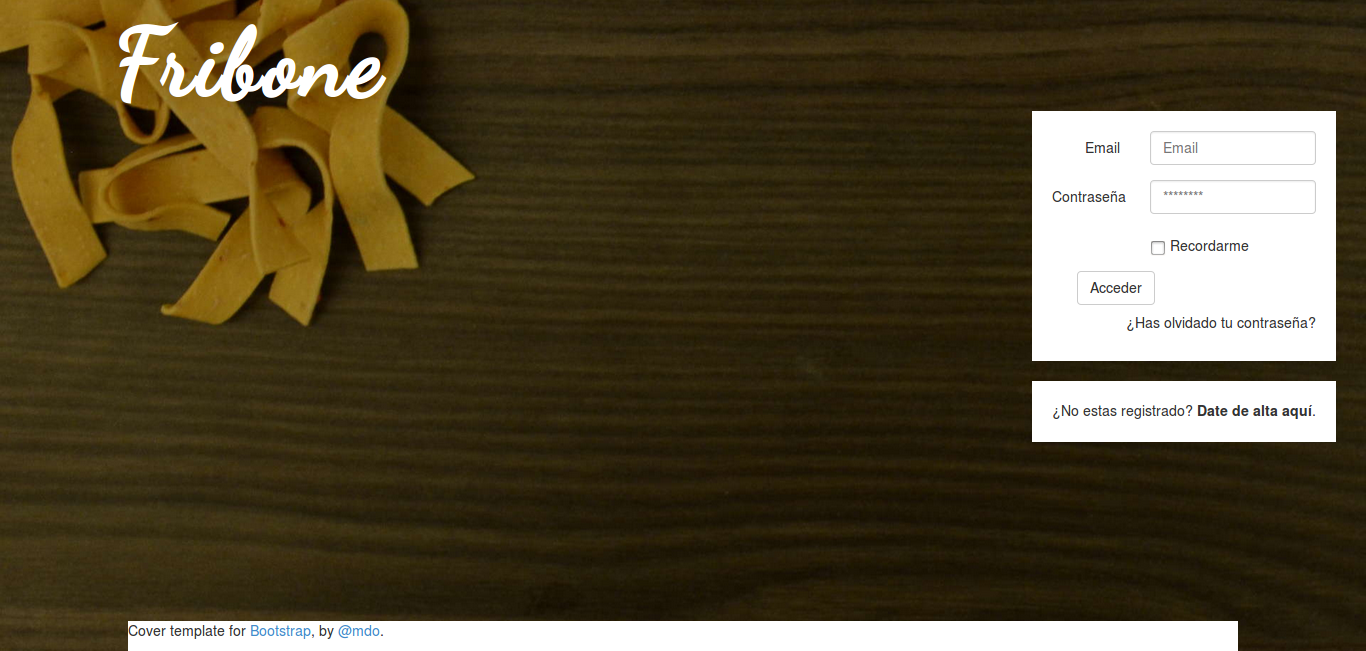
\includegraphics[keepaspectratio,width=0.9\textwidth]{fribone-web-home.png}
                \caption{Home aplicación web}\label{fig:fribone-web-home}
            \end{figure}


        \item Zona privada de usuario

            \begin{itemize}
                \item Frigorífico

                \item Compras realizadas

                \item Detalles de una compra

                \item Supermercados

                \item Vista de un supermercado

                \item Vista de los productos de un supermercado
            \end{itemize}
    \end{itemize}
